% !TeX encoding = UTF-8
% !TeX spellcheck = pt_BR
% !TeX root = 2024-JOAO-FERREIRA-TESE.tex
%---------------------------------------------------------------------

%---------------------------------------------------------------------
% Tese de Doutorado
% Autor: João Ferreira da Silva Júnior
%---------------------------------------------------------------------



%---------------------------------------------------------------------
\documentclass[
    %---------------------------------------------------------------------
    %% stock paper size
    a4paper,        % ABNT NBR 14724:2011
    %---------------------------------------------------------------------
    %% type size
    12pt,           % ABNT NBR 14724:2011
    %---------------------------------------------------------------------
    %% printing options
    % twoside,        % for when the document will be published with printing on both sides of the paper
    oneside,        % for when the document will be published with only one side of each sheet being printed on
    %
    % onecolumn,      % only one column of text on a page.
    % twocolumn,      % two equal width columns of text on a page.
    %
    openright,      % each chapter will start on a recto page.
    % openleft,       % each chapter will start on a verso page.
    % openany,        % a chapter may start on either a recto or verso page
    %
    final,          % for camera-ready copy of your labours.
    % draft,          % this marks overfull lines with black bars and enables some change marking to be shown
    % ms,             % this tries to make the document look as though it was prepared on a typewriter
    %
    % showtrims,      % this option prints marks at the corners of the sheet so that you can see where the stock must be trimmed to produce the final page size
    %---------------------------------------------------------------------
    %% other options
    % leqno,          % equations will be numbered at the left (the default is to number them at the right)
    % fleqn,          % displayed math environments will be indented an amount \mathindent from the left margin  (the default is to center the environments)
    %
    % openbib,        % each part of a bibliography entry will start on a new line, with second and succeding lines indented by \bibindent (the default is for an entry to run continuously with no indentations)
    %
    % article,        % typesetting simulates the article class, but the \chapter command is not disabled
    %---------------------------------------------------------------------
    %% abnTeX2 - opções específicas da classe abntex2: títulos de divisões em letras maiúsculas
    % chapter=TITLE,          % títulos de capítulos convertidos em letras maiúsculas
    % section=title,          % títulos de seções convertidos em letras maiúsculas
    % subsection=title,       % títulos de subseções convertidos em letras maiúsculas
    % subsubsection=title,    % títulos de subsubseções em letras maiúsculas
    % subsubsubsection=title, % títulos de subsubsubseções em letras maiúsculas
    %% definição do modelo do sumário
    sumario=tradicional, % abnt-6027-2012 ou tradicional
    %---------------------------------------------------------------------
    %% abnTeX2 - opções do pacote babel
    english,        % idioma adicional para hifenização
    french,         % idioma adicional para hifenização
    spanish,        % idioma adicional para hifenização
    brazil          % o último idioma é o principal do documento
    % ]{ppgec-abntex2} % Apesar da classe existir ela produz alguns bugs
    ]{abntex2}
%---------------------------------------------------------------------



%---------------------------------------------------------------------
%---------------------------------------------------------------------
%---------------------------------------------------------------------
%---------------------------------------------------------------------
%---------------------------------------------------------------------
% pacotes
\usepackage[utf8]{inputenc} % accept different input encodings (conversão automática dos acentos)
\usepackage[T1]{fontenc}    % standard package for selecting font encodings
%
\usepackage{adjustbox}      % the pack­age pro­vides sev­eral macros to ad­just boxed con­tent.
\usepackage{afterpage}      % execute command after the next page break
\usepackage{amsfonts}       % an extended set of fonts for use in mathematics
\usepackage{amsmath}        % extension package for LaTeX that provides various features to facilitate writing math formulas and to improve the typographical quality of their output
\usepackage{amssymb}        % math symbols defined by LaTeX package
% \usepackage{arydshln}       % draw dash-lines in array/tabular environments
\usepackage{babel}          % manages culturally-determined typographical (and other) rules, and hyphenation patterns for a wide range of languages
  \newcommand{\ingles}[1]{\foreignlanguage{english}{\emph{#1}}}
  \newcommand{\frances}[1]{\foreignlanguage{french}{\emph{#1}}}
  % \newcommand{\grego}[1]{\foreignlanguage{greek}{\emph{#1}}}
  \newcommand{\grego}[1]{\emph{#1}}
  \newcommand{\espanhol}[1]{\foreignlanguage{spanish}{\emph{#1}}}
  \newcommand{\portugues}[1]{\foreignlanguage{brazil}{\emph{#1}}}
% \usepackage{bbding}         % a symbol (dingbat) font and LaTeX macros for its use
\usepackage{booktabs}       % enhances the quality of tables in LATEX, providing extra commands as well as behind-the-scenes optimisation
% \usepackage{caption}        % provides many ways to customise the captions in floating environments like figure and table, and cooperates with many other packages.
% \usepackage{chemmacros}       % A collection of macros to support typesetting chemistry documents
% \usepackage{chngcntr}       % Change the resetting of counters.
  % \counterwithin{}{}        % Defines commands \counterwithin (which sets up a counter to be reset when another is incremented)
  % \counterwithout{equation}{chapter}  % Defines commands \counterwithout (which unsets such a relationship)
\usepackage{color}          % adding colors to your text is supported by the color package
\usepackage{courier}        % gives you Courier scaled at its normal size as the default Typewriter Font
\usepackage{enumitem}       % this package provides user control over the layout of the three basic list environments: enumerate, itemize and description
                            % http://linorg.usp.br/CTAN/macros/latex/contrib/enumitem/enumitem.pdf
% \usepackage{fancybox}       % implements commands for various boxes such as a box with round corners
% \usepackage{fancyhdr}       % pro­vides ex­ten­sive fa­cil­i­ties, both for con­struct­ing head­ers and foot­ers, and for con­trol­ling their use (for ex­am­ple, at times when LATEX would au­to­mat­i­cally change the head­ing style in use)
  % http://www.ctex.org/documents/packages/layout/fancyhdr.pdf
  % http://linorg.usp.br/CTAN/macros/latex/contrib/fancyhdr/fancyhdr.pdf
% \usepackage{filemod}        % provides macros to read and compare the modification dates of files
% \usepackage{framed}         % create framed, shaded, or differently highlighted regions that can break across pages
\usepackage{geometry}       % the pack­age pro­vides an easy and flex­i­ble user in­ter­face to cus­tomize page lay­out
  % http://texdoc.net/texmf-dist/doc/latex/geometry/geometry.pdf
  % https://pt.sharelatex.com/learn/Page_size_and_margins
  \geometry{
    % apenas a título de informação
    % 1cm = 28.3464567 pt
    % 1pt =  0.0352777778 cm
    %
    left=3cm,             % Margem esquerda:  left | lmargin | inner
    right=2cm,            % Margem direita:   right | rmargin | outer
    top=3cm,              % Margem superior:  top | tmargin
    bottom=2cm,           % Margem inferior:  bottom | bmargin
    % testar exaustivamente, pois poderá ocultar textos das margens
    % headheight=1.5cm,     % Altura total do cabeçalho
    % headsep=0.5cm,        % Sepação da base do cabeçalho ao corpo de texto
    % footskip=1cm,         % Distância entre a base do corpo de texto à base do rodapé
    % marginparwidth=36pt,  % Largura do margin note
    % marginparsep=8pt,     % Separação entre o parágrafo e a margin note
    % Opções para testes de modelo
    % showframe,            % the page frames are shown on every page
    % showcrop,             % prints crop marks at each corner of layout area on every page
  }
\usepackage{graphicx}       % enhanced support for graphics
\usepackage{hyperref}       % is used to handle cross-referencing commands in LaTeX to produce hypertext links in the document
\usepackage{indentfirst}    % indent first paragraph after section header
\usepackage{lastpage}       % reference the number of pages in your LATEX document through the introduction of a new label which can be referenced like \pageref{LastPage} to give a reference to the last page of a document
\usepackage{lipsum}         % this package gives you easy access to the Lorem Ipsum dummy text
\usepackage{listings}       % enables the user to typeset programs (programming code) within LATEX
  \lstset{postbreak=\raisebox{0ex}[0ex][0ex]{\ensuremath{\color{gray}\hookrightarrow\space}}}
  % TODO: Aqui tem um exemplo: https://github.com/abntex/abntex2/wiki/HowToFormatarCodigoFonte
  % TODO: https://tex.stackexchange.com/questions/64839/how-to-change-listing-caption
  \renewcommand{\lstlistingname}{Algoritmo}% Listing -> Algorithm
  \renewcommand{\lstlistlistingname}{Lista de algoritmos}% List of Listings -> List of Algorithms
\usepackage{lmodern}        % the Latin Modern family of fonts
\usepackage{longtable}      % allows you to write tables that continue to the next page
% \usepackage{makeidx}        % standard LaTeX package for creating indexes
% \usepackage{marginnote}     % provides the command \marginnote that may be used instead of \marginpar at almost every place where \marginpar cannot be used, e.g., inside floats, footnotes, or in frames made with the framed package
\usepackage{microtype}      % subliminal refinements towards typographical perfection
\usepackage{multicol}       % multicol defines a multicols environment which typesets text in multiple columns (up to a maximum of 10)
\usepackage{multirow}       % create tabular cells spanning multiple rows
% \usepackage{nameref}
% \usepackage{natbib}         % provides a package that implements both author-year and numbered references
% \usepackage{nomencl}        % produce lists of symbols as in nomenclature
\usepackage{paralist}       % provides some new list environments. Itemized and enumerated lists can be typesetted within paragraphs
\usepackage{pgfplots}       % draws high--quality function plots in normal or logarithmic scaling with a user-friendly interface directly in TeX
\usepackage{pgfplotstable}  % This package reads tab-separated numerical tables from input and generates code for pretty-printed LATEX-tabulars.
  \pgfplotsset{compat=1.14}
\usepackage{pgf-pie}        % provides the means to draw pie (and variant) charts, using PGF/TikZ
\usepackage{pdfpages}       % this package simplifies the inclusion of external multi-page PDF documents in LaTeX documents
% \usepackage{pifont}         % provides commands for Pi fonts (Dingbats, Symbol, etc...)
\usepackage{ragged2e}       % defines new commands \Centering, \RaggedLeft, and \RaggedRight and new environments Center, FlushLeft, and FlushRight, which set ragged text and are easily configurable to allow hyphenation
% \usepackage{showframe}      % makes the page margins visible and hence
\usepackage{siunitx}        % A comprehensive (SI) units package
\usepackage{soul}           % provides hyphenatable spacing out (letterspacing), underlining, striking out, etc., using the TeX hyphenation algorithm to find the proper hyphens automatically
% \usepackage{soulutf8}       % permit use of UTF-8 characters in soul
\usepackage{subfig}         % inclusão de Subfiguras https://www.ctan.org/pkg/subfig
\usepackage{tikz}           % for creating graphics programmatically
  \usetikzlibrary{arrows,automata,shadows}
\usepackage{times}          % select Adobe Times Roman (or equivalent) as default font
% \usepackage{titlesec}       % package providing an interface to sectioning commands for selection from various title styles. E.g., marginal titles and to change the font of all headings with a single command, also providing simple one-step page styles
  % \titleformat{command}[shape]{format}{label}{sep}{before}[after]
  % \titleformat{\part}[hang]{\bfseries\huge}{\thepart}{1em}{}[]
  % \titleformat{\chapter}[hang]{\bfseries\LARGE}{\thechapter}{1em}{}[]
  % \titleformat{\section}[hang]{\bfseries\Large\bfseries}{\thesection}{1em}{}
  % \titleformat{\subsection}[shape]{format}{label}{sep}{before}[after]
  % \titleformat{\subsubsection}[shape]{format}{label}{sep}{before}[after]
  % \titleformat{\paragraph}[shape]{format}{label}{sep}{before}[after]
  % \titleformat{\subparagraph}[shape]{format}{label}{sep}{before}[after]
% \usepackage{titletoc}
  % \titlecontents*{\subsection}[shape]{format}{label}{sep}{before}[after]
% \usepackage{todonotes}      % allows you to insert to–do items in your document
% \usepackage{wasysym}        % support file to use the WASY2 fonts
% \usepackage{wedn}           % font handwrite
  % inline font modify
  % \newcommand{\setfont}[2]{{\fontfamily{#1}\selectfont #2}}
  % Usage
  %\setfont{wedn}{Texto...}
\usepackage{xcolor}         % adding colors to your text is supported by the color package
%---------------------------------------------------------------------



%---------------------------------------------------------------------
%---------------------------------------------------------------------
%---------------------------------------------------------------------
%---------------------------------------------------------------------
%---------------------------------------------------------------------
% abnTeX2 - pacotes de citações
% Modelo da UPE
\usepackage[num,abnt-etal-list=0]{abntex2cite}	% Citações padrão ABNT, removendo et al na bibliografia
  \citebrackets[] % hack para colocar colchetes nas referencias.
\makeatletter
  \ifthenelse{\boolean{ABCIbiblabelonmargin}}
  {
    \renewcommand{\@biblabel}[1]%
    {\ifthenelse{\equal{#1}{}}{}{{\citenumstyle #1\hspace{\biblabelsep}}}}
  }
  {
    \renewcommand{\@biblabel}[1]%
    {%
      \ifthenelse{\equal{#1}{}}
      {}
      {%
        \def\biblabeltext{{\citenumstyle [#1]\hspace{\biblabelsep}}}%
        \settowidth{\ABCIauxlen}{\biblabeltext}%
        \ifthenelse{\lengthtest{\ABCIauxlen<\minimumbiblabelwidth}}
        {\setlength{\ABCIauxlen}{\minimumbiblabelwidth-\ABCIauxlen}}
        {\setlength{\ABCIauxlen}{0cm}}%
        {\biblabeltext\hspace{\ABCIauxlen}}%
      }%
    }%
  }
\makeatother
%---------------------------------------------------------------------



%---------------------------------------------------------------------
%---------------------------------------------------------------------
%---------------------------------------------------------------------
%---------------------------------------------------------------------
%---------------------------------------------------------------------
% Definição de macros de dados do documento
\titulo{Título do Trabalho}
\autor{O Grande Mestre do Universo}
\local{Recife}
\def\diadefesa{27}
\def\mesdefesa{julho}
\def\anodefesa{2024}
\data{\diadefesa~de~\mesdefesa~de~\anodefesa}
\orientador{O Supremo Senhor das Galáxias}
\coorientador{O Sábio Senhor das Estrelas}
\def\palavraschave{keyword;keyword;keyword}
\def\autorlattes{https://lattes.cnpq.br/}
\def\autorcitacoes{Silva Júnior, João Ferreira da}
\def\universidade{Universidade de Pernambuco}
\def\universidadesigla{UPE}
\def\logouniversidade{img/logo/logo-UPE.png}
\def\logouniversidadepb{img/logo/logo-UPE-PB.png}
\def\centro{Escola Politécnica de Pernambuco}
\def\logocentro{img/logo/logo-UPE-PPGEC.png}
\def\programa{Programa de Pós-Graduação em Engenharia da Computação}
\def\areaconcentracao{Computação}
\instituicao{%
    \SingleSpacing
    \universidade{}
    \par
    \centro{}
    \par
    \programa{}
}
% \tipotrabalho{Dissertação (Mestrado)}
% \tipotrabalho{Projeto de Tese (Doutorado)}
\tipotrabalho{Tese (Doutorado)}
\def\grau{Doutor}
\preambulo{\imprimirtipotrabalho{} submetida à avaliação pelo \programa{} da \universidade{} como parte dos requisitos para obtenção do grau de \grau{} em Engenharia da Computação.}
%
\author{\imprimirautor}
\title{\imprimirtitulo}
% \logo{}
% \institute{UPE}  % exclusiva do beamer
\date{\imprimirdata}
% \subject{}
%---------------------------------------------------------------------



%---------------------------------------------------------------------
%---------------------------------------------------------------------
%---------------------------------------------------------------------
%---------------------------------------------------------------------
%---------------------------------------------------------------------
% Configurações de espaçamento entre linhas e parágrafos de acordo com ABNT NBR 14724 - 2005
% \renewcommand{\baselinestretch}{1.5}        % todo o texto deve ser digitado ou datilografado com espaço 1,5
% \setlength{\tabcolsep}{0.5em}               % for the horizontal padding
% \renewcommand{\arraystretch}{1.2}           % for the vertical padding
\setlength{\parindent}{1.3cm}                 % indentation of the first line of a paragraph
\setlength{\parskip}{0.2cm}%\onelineskip}     % vertical spacing between paragraphs
% \setlength\afterchapskip{\lineskip}         % espaçamento entre os capítulos e o texto de 1.5 linhas
  % Nota: se realmente for utilizar esta regra, deverá constar imediatamente após a declaração de um capítulo de apêndice ou de anexo:
  % \chapter{Título de um anexo ou apêndice}
  % \setlength{\afterchapskip}{-\baselineskip}
%---------------------------------------------------------------------
% Evita divisão silábica das palavras
% badness is an integer from 0 to 10000 that is a measure of the quality of the spacing in any given box.
% \pretolerance=10000 % an integer parameter that is used in TeX's line breaking algorithm
% \tolerance=10000    % a parameter that tells TeX how much badness is allowable without error
%---------------------------------------------------------------------
% Configurações gerais do pacote abnTeX2
% \renewcommand{\ABNTEXpartfont}{\fontseries{b}\fontshape{n}\selectfont}
% \renewcommand{\ABNTEXpartfontsize}{\Large}
% \renewcommand{\ABNTEXchapterfont}{\fontseries{b}\fontshape{n}\selectfont}
% \renewcommand{\ABNTEXchapterfontsize}{\Large}
% \renewcommand{\ABNTEXsectionfont}{\fontseries{b}\fontshape{n}\selectfont}
% \renewcommand{\ABNTEXsectionfontsize}{\large}
% \renewcommand{\ABNTEXsubsectionfont}{\fontseries{m}\fontshape{n}\selectfont}
% \renewcommand{\ABNTEXsubsectionfontsize}{\large}
% \renewcommand{\ABNTEXsubsubsectionfont}{\fontfamily{cmr}\fontseries{m}\fontshape{it}\selectfont}
% \renewcommand{\ABNTEXsubsubsectionfontsize}{\normalsize}
%
% \newcommand{\refapendice}[1]{\hyperref[#1]{Apêndice~\ref{#1}}}
% \newcommand{\refanexo}[1]{\hyperref[#1]{Anexo~\ref{#1}}}
%
% Fontes das entradas do sumario
%
% \renewcommand{\cftpartfont}{\normalsize\bfseries}
% \renewcommand{\cftpartpagefont}{\normalsize\cftpartfont}
%
% \renewcommand{\cftchapterfont}{\normalsize\bfseries}
% \renewcommand{\cftchapterpagefont}{\normalsize\cftchapterfont}
% %
% \renewcommand{\cftsectionfont}{\normalsize\bfseries}
% \renewcommand{\cftsectionpagefont}{\normalsize\cftsectionfont}
%
% \renewcommand{\cftsubsectionfont}{\normalsize\normalfont}
% \renewcommand{\cftsubsectionpagefont}{\normalsize\cftsubsectionfont}
%
% \renewcommand{\cftsubsubsectionfont}{\normalsize\itshape}
% \renewcommand{\cftsubsubsectionpagefont}{\normalsize\cftsubsubsectionfont}
%
% \renewcommand{\cftparagraphfont}{\normalsize\itshape}
% \renewcommand{\cftparagraphpagefont}{\normalsize\cftparagraphfont}
%
% Nomes constantes do abnTeX2 em portugues (definicoes padroes)
% \renewcommand{\bibname}{REFER\^ENCIAS}
% \renewcommand{\anexosname}{ANEXOS}
% \renewcommand{\apendicesname}{AP\^ENDICES}
% Novo estilo usado apenas no cabeçalho da página em que se inicia o capítulo
% \makepagestyle{meuestilo_capitulo}
% \makeoddhead{meuestilo_capitulo}{}{}{\ABNTEXfontereduzida\thepage}
%---------------------------------------------------------------------



%---------------------------------------------------------------------
% definições pessoais
\definecolor{black}{rgb}{0.0, 0.0, 0.0}
\definecolor{white}{rgb}{255,255,255}
\definecolor{red}{rgb}{255,0,0}
\definecolor{green}{rgb}{0,255,0}
% \definecolor{blue}{RGB}{41,5,195} % Definição padrão da cor azul, todo mundo usa mas é feia
\definecolor{blue}{rgb}{0,0,255}
%---------------------------------------------------------------------
% Definições para forçar a hifenização de acordo com o idioma
% \hyphenation{á-gua}
% \hyphenation{pro-du-ção}
% \hyphenation{pro-du-\c{c}\~{a}o}
%---------------------------------------------------------------------



%---------------------------------------------------------------------
%---------------------------------------------------------------------
%---------------------------------------------------------------------
%---------------------------------------------------------------------
%---------------------------------------------------------------------
% Configurações do pacote hyperref, precisa estar aqui devido as macros de dados do documento
% Irá gerar marcadores no pdf, só é exibido em alguns leitores, e informações nas propriedades do documento
\makeatletter
\hypersetup{% http://www.tug.org/applications/hyperref/manual.html#x1-120003.8
  anchorcolor={black},                      % set color of anchors
  % backref=false,                            % do bibliographical back references
  baseurl={\autorlattes},                   % set base URL for document
  urlcolor={black},%{blue},                 % url color link
  % bookmarks={true},                         % make bookmarks
  bookmarksnumbered={false},                % put section numbers in bookmarks
  bookmarksopen={true},                     % open up bookmark tree
  bookmarksopenlevel={\maxdimen},           % level to which bookmarks are open
  bookmarksdepth,                           % <no-value>, <number>, <part,chapter,section,...>
  bookmarkstype={toc},                      % to specify which ‘toc’ file to mimic
  % breaklinks={false},                       % allow links to break over lines
  % citebordercolor=0 1 0,                    % color of border around cites
  citecolor={black},%{green},               % color of citation links
  colorlinks={true},
            % false,                          % color links
            % true,                           % (tex4ht, dviwindo)
  % debug=false,                              % provide details of anchors defined; same as verbose
  % destlabel=false,                          % destinations are named by the first \label after the anchor creation
  draft={false},                            % do not do any hyperlinking
  % filebordercolor=0 .5 .5,                  % color of border around file links
  filecolor={black},%{cyan},                % color of file links
  final={true},                             % opposite of option draft
  % frenchlinks=false,                        % use small caps instead of color for links
  % hyperfigures=false,                       % make figures hyper links
  % hyperfootnotes=true,                      % set up hyperlinked footnotes
  % hyperindex=true,                          % set up hyperlinked indices
  % linkbordercolor=1 0 0,                    % color of border around links
  linkcolor={black},%{red},                 % color of links
  % linktocpage={false},                      % make page number, not text, be link on TOC, LOF and LOT
  % menubordercolor=1 0 0,                    % color of border around menu links
  menucolor={black},%{red},                 % color for menu links
  pageanchor={true},                        % put an anchor on every page
  % pagebackref={true},                       % backreference by page number
  pdfauthor={\@author},                     % text for PDF Author field
  % pdfborder=0 0 1,                          % width of PDF link border
            % 0 0 0,                          % (colorlinks)
  % pdfcenterwindow=true,                     % position the document window in the center of the screen
  pdfcreator={LaTeX with hyperref package, feet: \@author},
                                            % text for PDF Creator field
  pdfdisplaydoctitle=true,                  % display document title instead of file name in title bar
  pdfkeywords={\palavraschave},
                                            % text for PDF Keywords field
  pdflang={pt-BR},                          % PDF language identifier (RFC 3066)
  pdfproducer={\@author},                   % text for PDF Producer field
  % pdfstartpage=1,                           % page at which PDF document opens
  pdfsubject={\imprimirpreambulo},          % text for PDF Subject field
  pdftitle={\@title}                        % text for PDF Title field
  }
\makeatother
%---------------------------------------------------------------------





%---------------------------------------------------------------------
%---------------------------------------------------------------------
%---------------------------------------------------------------------
%---------------------------------------------------------------------
%---------------------------------------------------------------------
% Posiciona figuras e tabelas no topo da página quando adicionadas sozinhas
% em um página em branco. Ver https://github.com/abntex/abntex2/issues/170
\makeatletter
\setlength{\@fptop}{5pt} % Set distance from top of page to first float
\makeatother
%---------------------------------------------------------------------





%---------------------------------------------------------------------
%---------------------------------------------------------------------
%---------------------------------------------------------------------
%---------------------------------------------------------------------
%---------------------------------------------------------------------
% Compila o índice, nomemclatura
\makeindex
% \makenomenclature % se ativar esta opção irá parar com a contagem de citações, bug do abntex
%---------------------------------------------------------------------





%---------------------------------------------------------------------
%---------------------------------------------------------------------
%---------------------------------------------------------------------
%---------------------------------------------------------------------
%---------------------------------------------------------------------
% Formato de cabeçalho/rodapé romano nos elementos pré-textuais

%% Novo estilo
\makepagestyle{estilo_pretextual} %%% escolha um nome
\makeevenhead{estilo_pretextual}{}{}{\ABNTEXfontereduzida \textit \thepage}
\makeoddhead{estilo_pretextual}{}{}{\ABNTEXfontereduzida \textit \thepage}

%---------------------------------------------------------------------
%% Customiza comando \pretextual
\renewcommand{\pretextual}{
  \aliaspagestyle{chapter}{estilo_pretextual}% customizing chapter pagestyle
  \pagestyle{estilo_pretextual}
  \aliaspagestyle{cleared}{empty}
  \aliaspagestyle{part}{estilo_pretextual}
}
%---------------------------------------------------------------------
% Ajusta a marca \textual para que a numeração volte a ser arábica
% nos elementos textuais
\let\oldtextual\textual        % copia o comando \textual anterior para \oldtextual
\renewcommand{\textual}{%
  \oldtextual%
  \pagenumbering{arabic} % volta à numeração arábica
}
%---------------------------------------------------------------------



%---------------------------------------------------------------------
%---------------------------------------------------------------------
%---------------------------------------------------------------------
%---------------------------------------------------------------------
%---------------------------------------------------------------------
\begin{document}



%---------------------------------------------------------------------
%---------------------------------------------------------------------
%---------------------------------------------------------------------
%---------------------------------------------------------------------
%---------------------------------------------------------------------
% Seleciona o idioma do documento (conforme pacotes do babel)
%\selectlanguage{english}
\selectlanguage{brazil}
% Retira espaço extra obsoleto entre as frases.
\frenchspacing
%---------------------------------------------------------------------



%---------------------------------------------------------------------
%---------------------------------------------------------------------
%---------------------------------------------------------------------
%---------------------------------------------------------------------
%---------------------------------------------------------------------
%---------------------------------------------------------------------
%---------------------------------------------------------------------
%---------------------------------------------------------------------
%---------------------------------------------------------------------
%---------------------------------------------------------------------
% Elementos pre-textuais
\pretextual{}



%---------------------------------------------------------------------
%---------------------------------------------------------------------
%---------------------------------------------------------------------
%---------------------------------------------------------------------
%---------------------------------------------------------------------
%% Capa externa OPCIONAL - ou capa dura - opção 1
%% Utilizada apenas quando for feita encadernação
%% Esta opção deverá ser utilizada no caso da capa dura ter sido feita externamente
% \renewcommand{\imprimircapa}{
%   \begin{capa}
%     \includepdf{inc/2024-JOAO-FERREIRA-TESE-CAPA-DURA.pdf}
%   \end{capa}
%   }
% \imprimircapa{}
% \clearpage % Não descomentar, este deve ficar comentado
%---------------------------------------------------------------------
%% Capa externa OPCIONAL - ou capa dura - opção 2
%% Utilizada apenas quando for feita encadernação
%% Esta opção deverá ser utilizada para criar a capa dura pelo próprio LaTeX
\renewcommand{\imprimircapa}{
  \begin{capa}
    \center{}
    %
    {\textbf{\MakeUppercase{\universidade}}}\\
    \vspace{0.25\onelineskip}
    {\textbf{\MakeUppercase{\centro}}}\\
    \vspace{0.25\onelineskip}
    {\textbf{\MakeUppercase{\programa}}}\\

    \vspace*{\fill}
    \begin{figure}[!h]
      \centering
      % \frame{% utilizar frame apenas para teste de leiaute
                       % trim={<left> <lower> <right> <upper>}
        % \includegraphics[trim={3cm 8cm 3cm 2.5cm},width=0.6\textwidth]{\logouniversidadepb}
        \includegraphics[width=0.6\textwidth,keepaspectratio]{\logouniversidadepb}
      % } % frame
    \end{figure}
    % \vspace*{\fill}

    % dados do trabalho e autor
    \vspace{0.5\onelineskip}
    {\textbf{\MakeUppercase{\imprimirtipotrabalho}}}\\
    \vspace{0.5\onelineskip}
    {\textbf{\imprimirtitulo}}\\
    \vspace*{\fill}
    {\textbf{\imprimirautor}}
  \end{capa}
  }
\imprimircapa{}
% \clearpage % deve ficar comentado
%---------------------------------------------------------------------



%---------------------------------------------------------------------
%---------------------------------------------------------------------
%---------------------------------------------------------------------
%---------------------------------------------------------------------
%---------------------------------------------------------------------
%% Capa editada, seguindo modelo do pacote abnTeX2
\renewcommand{\imprimircapa}{
    \begin{capa}
    \center{}
    %
    {\textbf{\MakeUppercase{\universidade}}}\\
    \vspace{0.25\onelineskip}
    {\textbf{\MakeUppercase{\centro}}}\\
    \vspace{0.25\onelineskip}
    {\textbf{\MakeUppercase{\programa}}}\\

    \vspace{8\onelineskip}
    {\textbf{\MakeUppercase{\imprimirautor}}}

    \vspace{5.5\onelineskip}
    \begin{center}
    % TODO: Verificar este alinhamento, o título deve ficar no centro da folha nesta página
    {\textbf{\MakeUppercase{\imprimirtitulo}}}
    \end{center}
    \vspace*{\fill}

    {\textbf{\MakeUppercase{\imprimirlocal}}}\\
    {\textbf{\MakeUppercase{\anodefesa}}}

    \vspace*{1cm}
    \end{capa}
}
\imprimircapa{}
% \clearpage % deve ficar comentado
%---------------------------------------------------------------------



%---------------------------------------------------------------------
%---------------------------------------------------------------------
%---------------------------------------------------------------------
%---------------------------------------------------------------------
%---------------------------------------------------------------------
%% Folha de rosto editada, seguindo modelo do pacote abnTeX2
\makeatletter
\renewcommand{\folhaderostocontent}{
    \center{}
    {\textbf{\MakeUppercase{\imprimirautor}}}\\

    % TODO: Verificar este alinhamento, o título deve ficar no centro da folha nesta página
    \vspace{19.65\onelineskip}
    % \vspace*{\fill}
    \begin{center}
        {\textbf{\MakeUppercase{\imprimirtitulo}}}
    \end{center}
    \vspace*{\fill}

    % preâmbulo
    \abntex@ifnotempty{\imprimirpreambulo}{%
        \hspace{0.5\textwidth}
        % \frame{% utilizar o frame para testes de leiaute
        % [pos][height][contentpos]{width}
        \begin{minipage}[t][][t]{0.47\textwidth}
            \SingleSpacing{}
            \imprimirpreambulo{}\\
            \\ \textbf{Área de Concentração}: \areaconcentracao.\\
            %
        \end{minipage}%
        % } % frame
    }%

    \justify\textbf{Orientadora}: Profª Drª \imprimirorientador{}
    \justify\textbf{Co-orientador}: Prof Dr \imprimircoorientador{}
    \vspace*{\fill}

    \center{}
    {\textbf{\MakeUppercase{\imprimirlocal}}}\\
    {\textbf{\MakeUppercase{\anodefesa}}}

    \vspace*{1cm}
}
\makeatother
\imprimirfolhaderosto{}   % para opção de impressão em um lado apenas oneside
% \imprimirfolhaderosto*  % para opção de impressão em frente e verso twoside
% \clearpage % deve ficar comentado
%---------------------------------------------------------------------



%---------------------------------------------------------------------
%---------------------------------------------------------------------
%---------------------------------------------------------------------
%---------------------------------------------------------------------
%---------------------------------------------------------------------
%% Ficha catalográfica editada, seguindo modelo do pacote abnTeX2
%% Ficha catalográfica - gerada pelo latex - opção 1
\begin{fichacatalografica}
    \vspace*{\fill}
    \begin{center}
        \rotatebox{45}{\Huge\MakeUppercase{Ficha modelo}}
    \end{center}
    \vspace*{\fill}
    \begin{center}
        \SingleSpacing{}
        \footnotesize{Catalogação na fonte}\\
        \footnotesize{Bibliotecária EDITAR NOME, CRB-9 / 9999}\\[0em]
        \begin{table}[h!]
            \begin{framed}
                \begin{tabular}{@{}p{1.0cm}p{14.0cm}@{}}
                A123b   & {\autorcitacoes{}.}\\[0.1em]
                        & {\setlength{\parindent}{1cm}\imprimirtitulo~/~\imprimirautor.~-~\anodefesa{}.}\\[0.1em]
                        & {\setlength{\parindent}{1cm}\pageref{LastPage} folhas, il., tabs., abr.., sigl.\@ simb.}\\[0.1em]
                        & \\[0.1em]
                        & {\setlength{\parindent}{1cm}Orientadora: \imprimirorientador{}.}\\[0.1em]
                        & {\setlength{\parindent}{1cm}Co-orientador: \imprimircoorientador{}.}\\[0.1em]
                        & ~\\[0.1em]
                        & {\setlength{\parindent}{1cm}\imprimirtipotrabalho{}~-~\universidade.~\centro.~\programa, \anodefesa{}.}\\[0.1em]
                        & {\setlength{\parindent}{1cm}Inclui Referências, Apêndices e Anexo.}\\[0.1em]
                        & \\[0.1em]
                        & \\[0.1em]
                        & {1. Keyword 1.\@ 2.\@ Keyword 2.\@ 3.\@ Keyword 3.\@ 4.\@ Keyword 4.\@ 5.\@ Keyword 5.\@ I.\@ \imprimirorientador{} (Orientadora).\@ II.\@ Título.}\\[0.1em]
                        & \\[0.1em]
                        & \hspace*{\fill}{\universidadesigla}\hspace*{6em}~\\[0.1em]
                        & \\[0.1em]
                        & {\setlength{\parindent}{1cm}999.9 CDD (22.\@ ed.)}\hspace*{\fill}{CODBIB/2024--07}\hspace*{4em}~{}
                \end{tabular}
            \end{framed}
        \end{table}
    \end{center}
\end{fichacatalografica}
% \clearpage % deve ficar comentado
%---------------------------------------------------------------------
%% Ficha catalográfica - pdf fornecido pela secretaria do programa - opção 2
% \begin{fichacatalografica}
%     % \vspace*{\fill} % A ficha deverá alinhar na base da página
%     % \includepdf{01-pre-textuais/ficha_catalografica.pdf}
% \end{fichacatalografica}
% \clearpage % deve ficar comentado
%---------------------------------------------------------------------



%---------------------------------------------------------------------
%---------------------------------------------------------------------
%---------------------------------------------------------------------
%---------------------------------------------------------------------
%---------------------------------------------------------------------
%% Folha de aprovação - utilizar um pdf fornecido pelo programa
\begin{folhadeaprovacao}
    \vspace*{\fill}
    \begin{center}
        \rotatebox{45}{\Huge\MakeUppercase{Folha de aprovação}}
    \end{center}
    \vspace*{\fill}
    %
    % \includepdf{inc/folha_aprovacao_sem_assinaturas.pdf}
    % \includepdf{inc/folha_aprovacao_com_assinaturas.pdf}
\end{folhadeaprovacao}
% \clearpage % deve ficar comentado
%---------------------------------------------------------------------



%---------------------------------------------------------------------
%---------------------------------------------------------------------
%---------------------------------------------------------------------
%---------------------------------------------------------------------
%---------------------------------------------------------------------
% Dedicatória
\begin{dedicatoria}
    \vspace*{\fill}
    \hspace{3.9cm}
    \begin{minipage}{10.5cm}
        \noindent
        \emph{Ao verme que primeiro roeu as frias carnes do meu cadáver dedico como saudosa lembrança estas memórias póstumas...}
    \end{minipage}
    \vspace*{1cm}
\end{dedicatoria}
% \clearpage % deve ficar comentado
%---------------------------------------------------------------------



%---------------------------------------------------------------------
%---------------------------------------------------------------------
%---------------------------------------------------------------------
%---------------------------------------------------------------------
%---------------------------------------------------------------------
% Agradecimentos
\begin{agradecimentos}
    Agradecimentos para: Deus, Pais, Irmãos, Esposa, Orientador, Amigos e Universidade.

    A Deus por me proporcionar perseverança durante toda a minha vida.

    Aos meus pais \ldots e \ldots pelo apoio e incentivo que serviram de alicerce para as minhas realizações.

    Aos meus irmãos \ldots e \ldots pela amizade e atenção dedicadas quando sempre precisei.

    À minha querida esposa \ldots pelo seu amor incondicional e por compreender minha dedicação ao projeto de pesquisa.

    Ao meu professor orientador \ldots pelas valiosas contribuições dadas durante todo o processo.

    A todos os meus amigos do curso de graduação que compartilharam dos inúmeros desafios que enfrentamos, sempre com o espírito colaborativo.

    Também quero agradecer à Universidade \ldots e o seu corpo docente que demonstrou estar comprometido com a qualidade e excelência do ensino.
\end{agradecimentos}
% \clearpage % deve ficar comentado
%---------------------------------------------------------------------



%---------------------------------------------------------------------
%---------------------------------------------------------------------
%---------------------------------------------------------------------
%---------------------------------------------------------------------
%---------------------------------------------------------------------
% Epígrafe
\begin{epigrafe}
    \vspace*{0.4\textheight}
    \begin{center}
        \textcolor{lightgray}{\( \therefore \)}
    \end{center}
    \vspace*{\fill}

    \hspace{3.9cm}
    \begin{minipage}{10.5cm}
        \noindent
        \raggedleft{}
        \emph{``Vigie seus pensamentos, porque eles se tornarão palavras.\\
            Vigie suas palavras, porque elas se tornarão seus hábitos.\\
            Vigie seus hábitos, porque eles se tornarão seu caráter.\\
            Vigie seu caráter, porque ele será o seu destino.''}\\
        \raggedleft{} \emph{(Frank Outlaw)}
    \end{minipage}

    \vspace*{1cm}
\end{epigrafe}
% \clearpage % deve ficar comentado
%---------------------------------------------------------------------



%---------------------------------------------------------------------
%---------------------------------------------------------------------
%---------------------------------------------------------------------
%---------------------------------------------------------------------
%---------------------------------------------------------------------
% Resumos
%---------------------------------------------------------------------
% Resumo em português
\begin{resumo}
    % Contexto
    \lipsum[4]
    % Motivação
    \lipsum[4]
    % Objetivo geral
    \lipsum[4]
    % Procedimentos e métodos
    \lipsum[4]
    % Resultados obtidos
    \lipsum[4]
    % Discussões
    \lipsum[4]
    % \vspace*{\onelineskip}

    \noindent
    \textbf{Palavras-chave}: Palavra-chave 1. Palavra-chave 2. Palavra-chave 3.
\end{resumo}
\clearpage{}
%---------------------------------------------------------------------
% Resumo em inglês
\begin{resumo}[Abstract]
    \begin{otherlanguage*}{english}
        % Contexto
        \lipsum[4]
        % Motivação
        \lipsum[4]
        % Objetivo geral
        \lipsum[4]
        % Procedimentos e métodos
        \lipsum[4]
        % Resultados obtidos
        \lipsum[4]
        % Discussões
        \lipsum[4]
        % \vspace*{\onelineskip}

        \noindent
        \textbf{Keywords}: Keyword 1. Keyword 2. Keyword 3.
    \end{otherlanguage*}
\end{resumo}
\clearpage{}
%---------------------------------------------------------------------



%---------------------------------------------------------------------
%---------------------------------------------------------------------
%---------------------------------------------------------------------
%---------------------------------------------------------------------
%---------------------------------------------------------------------
% Lista de ilustracoes
\pdfbookmark[0]{\listfigurename}{lof}
    \listoffigures*
\clearpage{}
%---------------------------------------------------------------------



%---------------------------------------------------------------------
%---------------------------------------------------------------------
%---------------------------------------------------------------------
%---------------------------------------------------------------------
%---------------------------------------------------------------------
% Lista de tabelas
\pdfbookmark[0]{\listtablename}{lot}
    \listoftables*
\clearpage{}
%---------------------------------------------------------------------



%---------------------------------------------------------------------
%---------------------------------------------------------------------
%---------------------------------------------------------------------
%---------------------------------------------------------------------
%---------------------------------------------------------------------
% Lista de algoritmos
% TODO: Ocorreram alguns bugs que não consegui corrigir, mas teste, se der certo, então ótimo!
% TODO: https://tex.stackexchange.com/questions/64839/how-to-change-listing-caption
% Preferi omitir esta seção, já que não é obrigatória
\pdfbookmark[0]{\lstlistlistingname}{lot}
    \begin{KeepFromToc}
        \lstlistoflistings{}
    \end{KeepFromToc}
% \cleardoublepage{}
\clearpage{}
%---------------------------------------------------------------------



%---------------------------------------------------------------------
%---------------------------------------------------------------------
%---------------------------------------------------------------------
%---------------------------------------------------------------------
%---------------------------------------------------------------------
% Lista de abreviaturas e siglas
\begin{siglas}%
    \item[]
    \begin{alineas}[
        font=\normalfont,
        format=\normalsize,
        align=parleft,
        itemsep=1ex,
        % Opções para delimitação dos espaçamentos
        %% \leftmargin + \itemindent = \labelindent + \labelwidth + \labelsep
        % leftmargin=4em,itemindent=0em,labelindent=0em,labelwidth=10em,labelsep=0em]
        leftmargin=-2em,itemindent=0em,labelindent=0em,labelwidth=6em,labelsep=0em]
        % Modelo para o alinhamento
        % Lista de itens deverá estar ordenada alfabeticamente
        % \item[mmmmmmmmmm] mmmmmmmmmm mmmmmmmmmm mmmmmmmmmm m mmmmmmmmm mmmmmmmmmm mmmmmmmmmm
        \item[ACP]          Análise de Componentes Principais
        \item[AFI]          Análise da Frequência Instantânea
        \item[CAPES]        Coordenação de Aperfeiçoamento de Pessoal de Nível Superior
        \item[CNPQ]         Conselho Nacional de Desenvolvimento Científico e Tecnológico
        \item[EQM]          Erro Quadrático Médio
        \item[IBM]          \ingles{International Business Machines}
        \item[IEEE]         \ingles{Institute of Electrical and Electronics Engineers}
        \item[IoT]          \ingles{Internet of Things}
        \item[MSL]          Mapeamento Sistemático da Literatura
        \item[OMS]          Organização Mundial da Saúde
        \item[ONU]          Organização das Nações Unidas
        \item[PCA]          \ingles{Principal Component Analisys}
    \end{alineas}
\end{siglas}
\clearpage{}
%---------------------------------------------------------------------



%---------------------------------------------------------------------
%---------------------------------------------------------------------
%---------------------------------------------------------------------
%---------------------------------------------------------------------
%---------------------------------------------------------------------
% Lista de símbolos
\begin{simbolos}
    \item[]
    \begin{alineas}[
        font=\normalfont,
        format=\normalsize,
        align=parleft,
        itemsep=1ex,
        % Opções para delimitação dos espaçamentos
        %% \leftmargin + \itemindent = \labelindent + \labelwidth + \labelsep
        % leftmargin=4em,itemindent=0em,labelindent=0em,labelwidth=10em,labelsep=0em]
        leftmargin=-2em,itemindent=0em,labelindent=0em,labelwidth=6em,labelsep=0em]
        % Modelo para o alinhamento
        % Lista de itens deverá estar ordenada alfabeticamente
        % \item[mmmmmmmmmm] mmmmmmmmmm mmmmmmmmmm mmmmmmmmmm m mmmmmmmmm mmmmmmmmmm mmmmmmmmmm
        \item[\(A\)]        Ampere
        \item[\(DC\)]       \ingles{Direct Current}
        \item[\(GHz\)]      Gigahertz
        \item[\(H\)]        Transformada de Hilbert
        \item[\(|H|\)]      Transformada de Hilbert Normalizada
        \item[\(KB\)]       Kilobyte
        \item[\(Kbps\)]     Kilobit por segundo
        \item[\(L/min\)]    Litros por minuto
        \item[\(mA\)]       Miliampere
        \item[\(MHz\)]      Megahertz
        \item[\(MPa\)]      Megapascal
        \item[\(ms\)]       Milissegundo
        \item[º\(C\)]       Grau centígrado, ou grau Celsius
        \item[\(QD\)]       Quadratura Direta
        \item[\(TEO\)]      \ingles{Teager Energy Operator}
        \item[\(V\)]        Volt
    \end{alineas}
\end{simbolos}
\clearpage{}
%---------------------------------------------------------------------



%---------------------------------------------------------------------
%---------------------------------------------------------------------
%---------------------------------------------------------------------
%---------------------------------------------------------------------
%---------------------------------------------------------------------
% Incluir sumário
\pdfbookmark[0]{\contentsname}{toc}
    \tableofcontents*
\clearpage{}
%---------------------------------------------------------------------



%---------------------------------------------------------------------
%---------------------------------------------------------------------
%---------------------------------------------------------------------
%---------------------------------------------------------------------
%---------------------------------------------------------------------
%---------------------------------------------------------------------
%---------------------------------------------------------------------
%---------------------------------------------------------------------
%---------------------------------------------------------------------
%---------------------------------------------------------------------
% elementos textuais
\textual{}
%%usar o estilo criado nas páginas textuais
\pagestyle{simple}
% \makeoddhead{simple}{}{}{\ABNTEXfontereduzida\thepage}
\aliaspagestyle{chapter}{simple}
%---------------------------------------------------------------------



%---------------------------------------------------------------------
%---------------------------------------------------------------------
%---------------------------------------------------------------------
%---------------------------------------------------------------------
%---------------------------------------------------------------------
%---------------------------------------------------------------------
%---------------------------------------------------------------------
%---------------------------------------------------------------------
%---------------------------------------------------------------------
%---------------------------------------------------------------------
% !TeX encoding = UTF-8
% !TeX spellcheck = pt_BR
% !TeX root = 2024-JOAO-FERREIRA-TESE.tex
%---------------------------------------------------------------------

%---------------------------------------------------------------------
% Tese de Doutorado
% Autor: João Ferreira da Silva Júnior
%---------------------------------------------------------------------



%---------------------------------------------------------------------
%---------------------------------------------------------------------
%---------------------------------------------------------------------
%---------------------------------------------------------------------
%---------------------------------------------------------------------
%---------------------------------------------------------------------
%---------------------------------------------------------------------
%---------------------------------------------------------------------
%---------------------------------------------------------------------
%---------------------------------------------------------------------
\chapter[Introdução]{Introdução}\label{cha:introducao}
    \chapterprecishere{
        \hspace{.2\textwidth}
        \hspace*{\fill}
        \begin{minipage}{.6\textwidth}
            \SingleSpace
            \raggedleft
            \noindent
            ``A luz sempre encontrará aqueles que a procuram.''\\
            (Autor desconhecido)
            % \emph{}
        \end{minipage}
    }
    \lipsum[1]
%---------------------------------------------------------------------



%---------------------------------------------------------------------
%---------------------------------------------------------------------
%---------------------------------------------------------------------
%---------------------------------------------------------------------
%---------------------------------------------------------------------
% \vspace*{0.2cm}
\section[Subseção 1]{Subseção 1}\label{sec:introducao-subsecao1}
    \lipsum[1]
%---------------------------------------------------------------------



%---------------------------------------------------------------------
% \vspace*{0.2cm}
\subsection[Sub-subseção 1]{Sub-subseção 1}\label{subsec:introducao-subsubsecao1}
    \lipsum[1]

    A seguir dois exemplos de tabela baseados no modelo do IBGE, o primeiro utilizado uma imagem para apresentar os dados, na \autoref{tab:pokemon-imagem}, e o segundo exemplo de fato trazendo os dados no formato de tabela, na \autoref{tab:pokemon-tabela}.
    \begin{table}[htb]
        \IBGEtab{%
            \caption{Trilha Sonora Pokémon --- em imagem}\label{tab:pokemon-imagem}
        }
        {%
            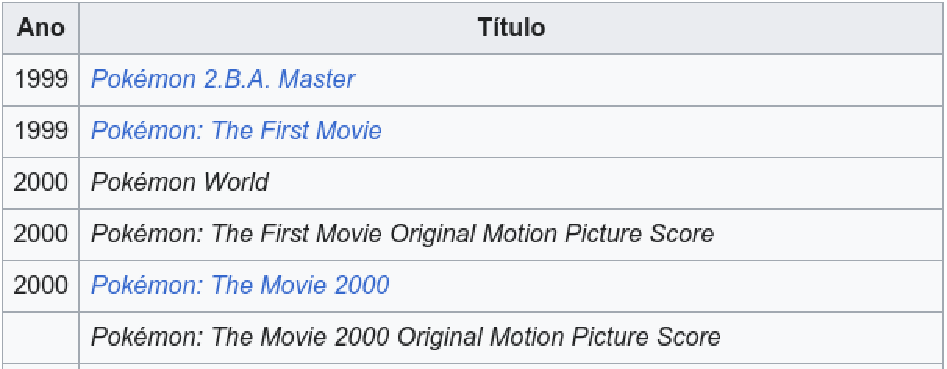
\includegraphics[width=0.8\textwidth,keepaspectratio]{img/01-introducao/pokemon.pdf}
        }
        {%
            \fonte{Adaptado de \citeonline{Wikipedia2005}.}
        }
    \end{table}

    \begin{table}[htb]
        \IBGEtab{%
            \caption{Trilha Sonora Pokémon --- em tabela}\label{tab:pokemon-tabela}
        }
        {%
            \begin{tabular}{cl}
                \toprule
                \textbf{Ano}    & \textbf{Título}                                           \\
                \midrule\midrule
                1999            & Pokémon 2.B.A. Master                                     \\
                1999            & Pokémon: The First Movie                                  \\
                2000            & Pokémon World                                             \\
                2000            & Pokémon: The First Movie Original Motion Picture Score    \\
                2000            & Pokémon: The Movie 2000                                   \\
                                & Pokémon: The Movie 2000 Original Motion Picture Score     \\
                \bottomrule
            \end{tabular}
        }
        {%
            \fonte{Adaptado de \citeonline{Wikipedia2005}.}
        }
    \end{table}

    Também é possível utilizar parágrafos dentro da tabela para posicionar os dados, que ficarão automaticamente alinhados à esquerda.
    \begin{table}[htb]
        \IBGEtab{%
            \caption{Trilha Sonora Pokémon --- em tabela com parágrafo}\label{tab:pokemon-tabela-paragrafo}
        }
        {%
            \begin{tabular}{cp{13.0cm}}
                \toprule
                \textbf{Ano}    & \textbf{Título}                                           \\
                \midrule\midrule
                1999            & Pokémon 2.B.A. Master                                     \\
                1999            & Pokémon: The First Movie                                  \\
                2000            & Pokémon World                                             \\
                2000            & Pokémon: The First Movie Original Motion Picture Score    \\
                2000            & Pokémon: The Movie 2000                                   \\
                & Pokémon: The Movie 2000 Original Motion Picture Score     \\
                \bottomrule
            \end{tabular}
        }
        {%
            \fonte{Adaptado de \citeonline{Wikipedia2005}.}
        }
    \end{table}

%---------------------------------------------------------------------



%---------------------------------------------------------------------
%---------------------------------------------------------------------
%---------------------------------------------------------------------
%---------------------------------------------------------------------
%---------------------------------------------------------------------
% \vspace*{0.2cm}
\section[Subseção 2]{Subseção 2}\label{sec:introducao-subsecao2}
    \lipsum[1]

    \begin{figure}[htb]
        \centering
        \caption{Hybrid Artificial Neural Network}\label{fig:hybrid-artificial-nn}
        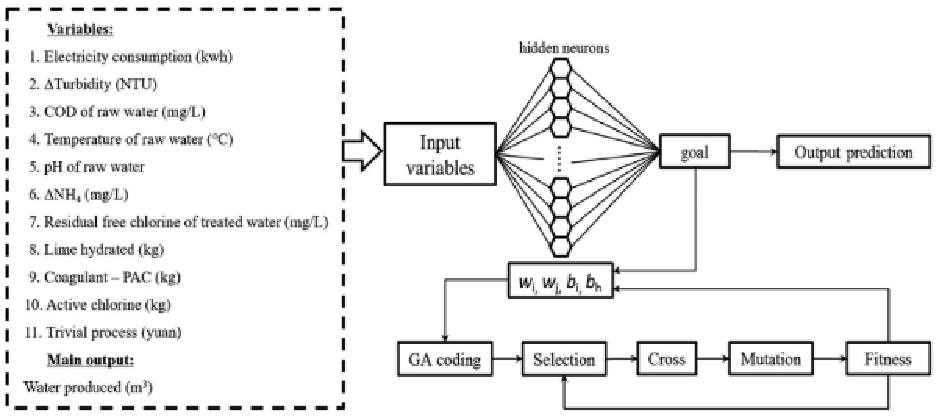
\includegraphics[width=0.8\textwidth,keepaspectratio]{img/01-introducao/hybrid-artificial-nn.pdf}
        %
        \fonte{Adaptado de \citeonline{Zhang2019}.}
        %
        % \nota[]
        \nota[]{%
            \parbox{0.8\textwidth}{%
                Aqui segue uma nota explicativa sobre o conteúdo e propósito da imagem.
            }
        }
    \end{figure}

    \lipsum[2]

    \lstinputlisting[%
        label=codigo-python,
        caption=codigo-python,
        language=Python,
        basicstyle=\tiny\ttfamily, breakatwhitespace=false,
        breaklines=true, breakatwhitespace=false, prebreak=\space, postbreak=\space
        showspaces=false, showstringspaces=false, showtabs=false,
        frame=single, rulecolor=\color{gray}, keywordstyle=,
        numbers=left, numbersep=5pt, numberstyle=\tiny\color{gray}, stepnumber=1
    ]{inc/codigo-python.py}

%---------------------------------------------------------------------
% !TeX encoding = UTF-8
% !TeX spellcheck = pt_BR
% !TeX root = 2024-JOAO-FERREIRA-TESE.tex
%---------------------------------------------------------------------

%---------------------------------------------------------------------
% Tese de Doutorado
% Autor: João Ferreira da Silva Júnior
%---------------------------------------------------------------------



%---------------------------------------------------------------------
%---------------------------------------------------------------------
%---------------------------------------------------------------------
%---------------------------------------------------------------------
%---------------------------------------------------------------------
%---------------------------------------------------------------------
%---------------------------------------------------------------------
%---------------------------------------------------------------------
%---------------------------------------------------------------------
%---------------------------------------------------------------------
\chapter[Desenvolvimento]{Desenvolvimento}\label{cha:desenvolvimento}
    \chapterprecishere{
        \hspace{.2\textwidth}
        \hspace*{\fill}
        \begin{minipage}{.6\textwidth}
            \SingleSpace
            \raggedleft
            \noindent
            ``A luz sempre encontrará aqueles que a procuram.''\\
            (Autor desconhecido)
            % \emph{}
        \end{minipage}
    }
    \lipsum[1]
%---------------------------------------------------------------------



%---------------------------------------------------------------------
%---------------------------------------------------------------------
%---------------------------------------------------------------------
%---------------------------------------------------------------------
%---------------------------------------------------------------------
% \vspace*{0.2cm}
\section[Subseção 1]{Subseção 1}\label{sec:desenvolvimento-subsecao1}
    \lipsum[1]
%---------------------------------------------------------------------



%---------------------------------------------------------------------
% \vspace*{0.2cm}
\subsection[Sub-subseção 1]{Sub-subseção 1}\label{subsec:desenvolvimento-subsubsecao1}
    \lipsum[1]
%---------------------------------------------------------------------



%---------------------------------------------------------------------
%---------------------------------------------------------------------
%---------------------------------------------------------------------
%---------------------------------------------------------------------
%---------------------------------------------------------------------
% \vspace*{0.2cm}
\section[Subseção 2]{Subseção 2}\label{sec:desenvolvimento-subsecao2}
    \lipsum[1]
%---------------------------------------------------------------------
% !TeX encoding = UTF-8
% !TeX spellcheck = pt_BR
% !TeX root = 2024-JOAO-FERREIRA-TESE.tex
%---------------------------------------------------------------------

%---------------------------------------------------------------------
% Tese de Doutorado
% Autor: João Ferreira da Silva Júnior
%---------------------------------------------------------------------



%---------------------------------------------------------------------
%---------------------------------------------------------------------
%---------------------------------------------------------------------
%---------------------------------------------------------------------
%---------------------------------------------------------------------
%---------------------------------------------------------------------
%---------------------------------------------------------------------
%---------------------------------------------------------------------
%---------------------------------------------------------------------
%---------------------------------------------------------------------
\chapter[Conclusão]{Conclusão}\label{cha:conclusao}
    \chapterprecishere{
        \hspace{.2\textwidth}
        \hspace*{\fill}
        \begin{minipage}{.6\textwidth}
            \SingleSpace
            \raggedleft
            \noindent
            ``A luz sempre encontrará aqueles que a procuram.''\\
            (Autor desconhecido)
            % \emph{}
        \end{minipage}
    }
    \lipsum[1]
%---------------------------------------------------------------------



%---------------------------------------------------------------------
%---------------------------------------------------------------------
%---------------------------------------------------------------------
%---------------------------------------------------------------------
%---------------------------------------------------------------------
% \vspace*{0.2cm}
\section[Subseção 1]{Subseção 1}\label{sec:conclusao-subsecao1}
    \lipsum[1]
%---------------------------------------------------------------------



%---------------------------------------------------------------------
% \vspace*{0.2cm}
\subsection[Sub-subseção 1]{Sub-subseção 1}\label{subsec:conclusao-subsubsecao1}
    \lipsum[1]
%---------------------------------------------------------------------



%---------------------------------------------------------------------
%---------------------------------------------------------------------
%---------------------------------------------------------------------
%---------------------------------------------------------------------
%---------------------------------------------------------------------
% \vspace*{0.2cm}
\section[Subseção 2]{Subseção 2}\label{sec:conclusao-subsecao2}
    \lipsum[1]
%---------------------------------------------------------------------
%---------------------------------------------------------------------



%---------------------------------------------------------------------
%---------------------------------------------------------------------
%---------------------------------------------------------------------
%---------------------------------------------------------------------
%---------------------------------------------------------------------
%---------------------------------------------------------------------
%---------------------------------------------------------------------
%---------------------------------------------------------------------
%---------------------------------------------------------------------
%---------------------------------------------------------------------
% elementos pós-textuais
\postextual{}
%---------------------------------------------------------------------



%---------------------------------------------------------------------
%---------------------------------------------------------------------
%---------------------------------------------------------------------
%---------------------------------------------------------------------
%---------------------------------------------------------------------
% Referências bibliográficas
\bibliography{library}
%---------------------------------------------------------------------



%---------------------------------------------------------------------
%---------------------------------------------------------------------
%---------------------------------------------------------------------
%---------------------------------------------------------------------
%---------------------------------------------------------------------
% Glossário
% Consulte o manual da classe abntex2 para orientações sobre o glossário.
% É o inferno na terra fazer isso funcionar, boa sorte!
% Mas, não é obrigatório
% \glossary{}
%---------------------------------------------------------------------



%---------------------------------------------------------------------
%---------------------------------------------------------------------
%---------------------------------------------------------------------
%---------------------------------------------------------------------
%---------------------------------------------------------------------
%---------------------------------------------------------------------
%---------------------------------------------------------------------
%---------------------------------------------------------------------
%---------------------------------------------------------------------
%---------------------------------------------------------------------
% Apêndices
\begin{apendicesenv}

    % Imprime uma página indicando o início dos apêndices
    \partapendices{}

    % \include{2024-JOAO-FERREIRA-TESE-APENDICE-A}

    % \include{2024-JOAO-FERREIRA-TESE-APENDICE-A}

\end{apendicesenv}
%---------------------------------------------------------------------



%---------------------------------------------------------------------
%---------------------------------------------------------------------
%---------------------------------------------------------------------
%---------------------------------------------------------------------
%---------------------------------------------------------------------
%---------------------------------------------------------------------
%---------------------------------------------------------------------
%---------------------------------------------------------------------
%---------------------------------------------------------------------
%---------------------------------------------------------------------
% Anexos
\begin{anexosenv}

    % Imprime uma página indicando o início dos anexos
    \partanexos{}

    % \include{2024-JOAO-FERREIRA-TESE-ANEXO-A}

\end{anexosenv}
%---------------------------------------------------------------------



%---------------------------------------------------------------------
%---------------------------------------------------------------------
%---------------------------------------------------------------------
%---------------------------------------------------------------------
%---------------------------------------------------------------------
%---------------------------------------------------------------------
%---------------------------------------------------------------------
%---------------------------------------------------------------------
%---------------------------------------------------------------------
%---------------------------------------------------------------------
% Finalização
\phantompart
\printindex
%---------------------------------------------------------------------



\end{document}
